\subsection{Software in the Loop (SITL)}

The SITL simulation conducted in this semester was showcased through a series of three experiments, each designed to test a specific aspect of the autonomous drone's capabilities. The first experiment focused on waypoint control, where waypoints were set with precise coordinates including position, altitude, and orientation utilizing set{\_}destination() function in the GNC library. The waypoints were designated as (5, 5), (15, 5), (15, -5), and (5, -5), with an altitude of 2 meters. At each waypoint, the orientations were set to 90, 180, 270, and 360 degrees, respectively. The drone successfully executed the task, initiating takeoff and then navigating to each waypoint in the prescribed sequence. A demonstration of a square flight trajectory with 4 waypoints is shown in Fig. \ref{fig3d1}. This outcome highlights the precision of the drone's flight path control and the efficacy of the GNC library.


\begin{figure}[H]
    \centerline{\includegraphics[width=0.5\textwidth]{Figures/Results/waypoints.jpeg}}
    \caption{Navigation through 4 Waypoints in Sequence (camera positioned vertically downward): 1 (top left) $\rightarrow$ 2 (top right) $\rightarrow$ 3 (bottom left) $\rightarrow$ 4 (bottom right)}
    \label{fig3d1}
\end{figure}

The second experiment evaluated the drone's human detection system. Four human models, featuring various genders and poses, were introduced into the simulation environment. To further challenge the system, interference objects were also added to the environment, simulating potential real-life distractions and occlusions that the drone might encounter. The OpenCV DNN module, equipped with the YOLO algorithm, was utilized to detect and count the number of humans in the frame. The experiment was successful as shown in Fig. \ref{fig3d2}. The system accurately identified and counted the human models, demonstrating the reliability of the object detection implementation.

\begin{figure}[H]
    \centerline{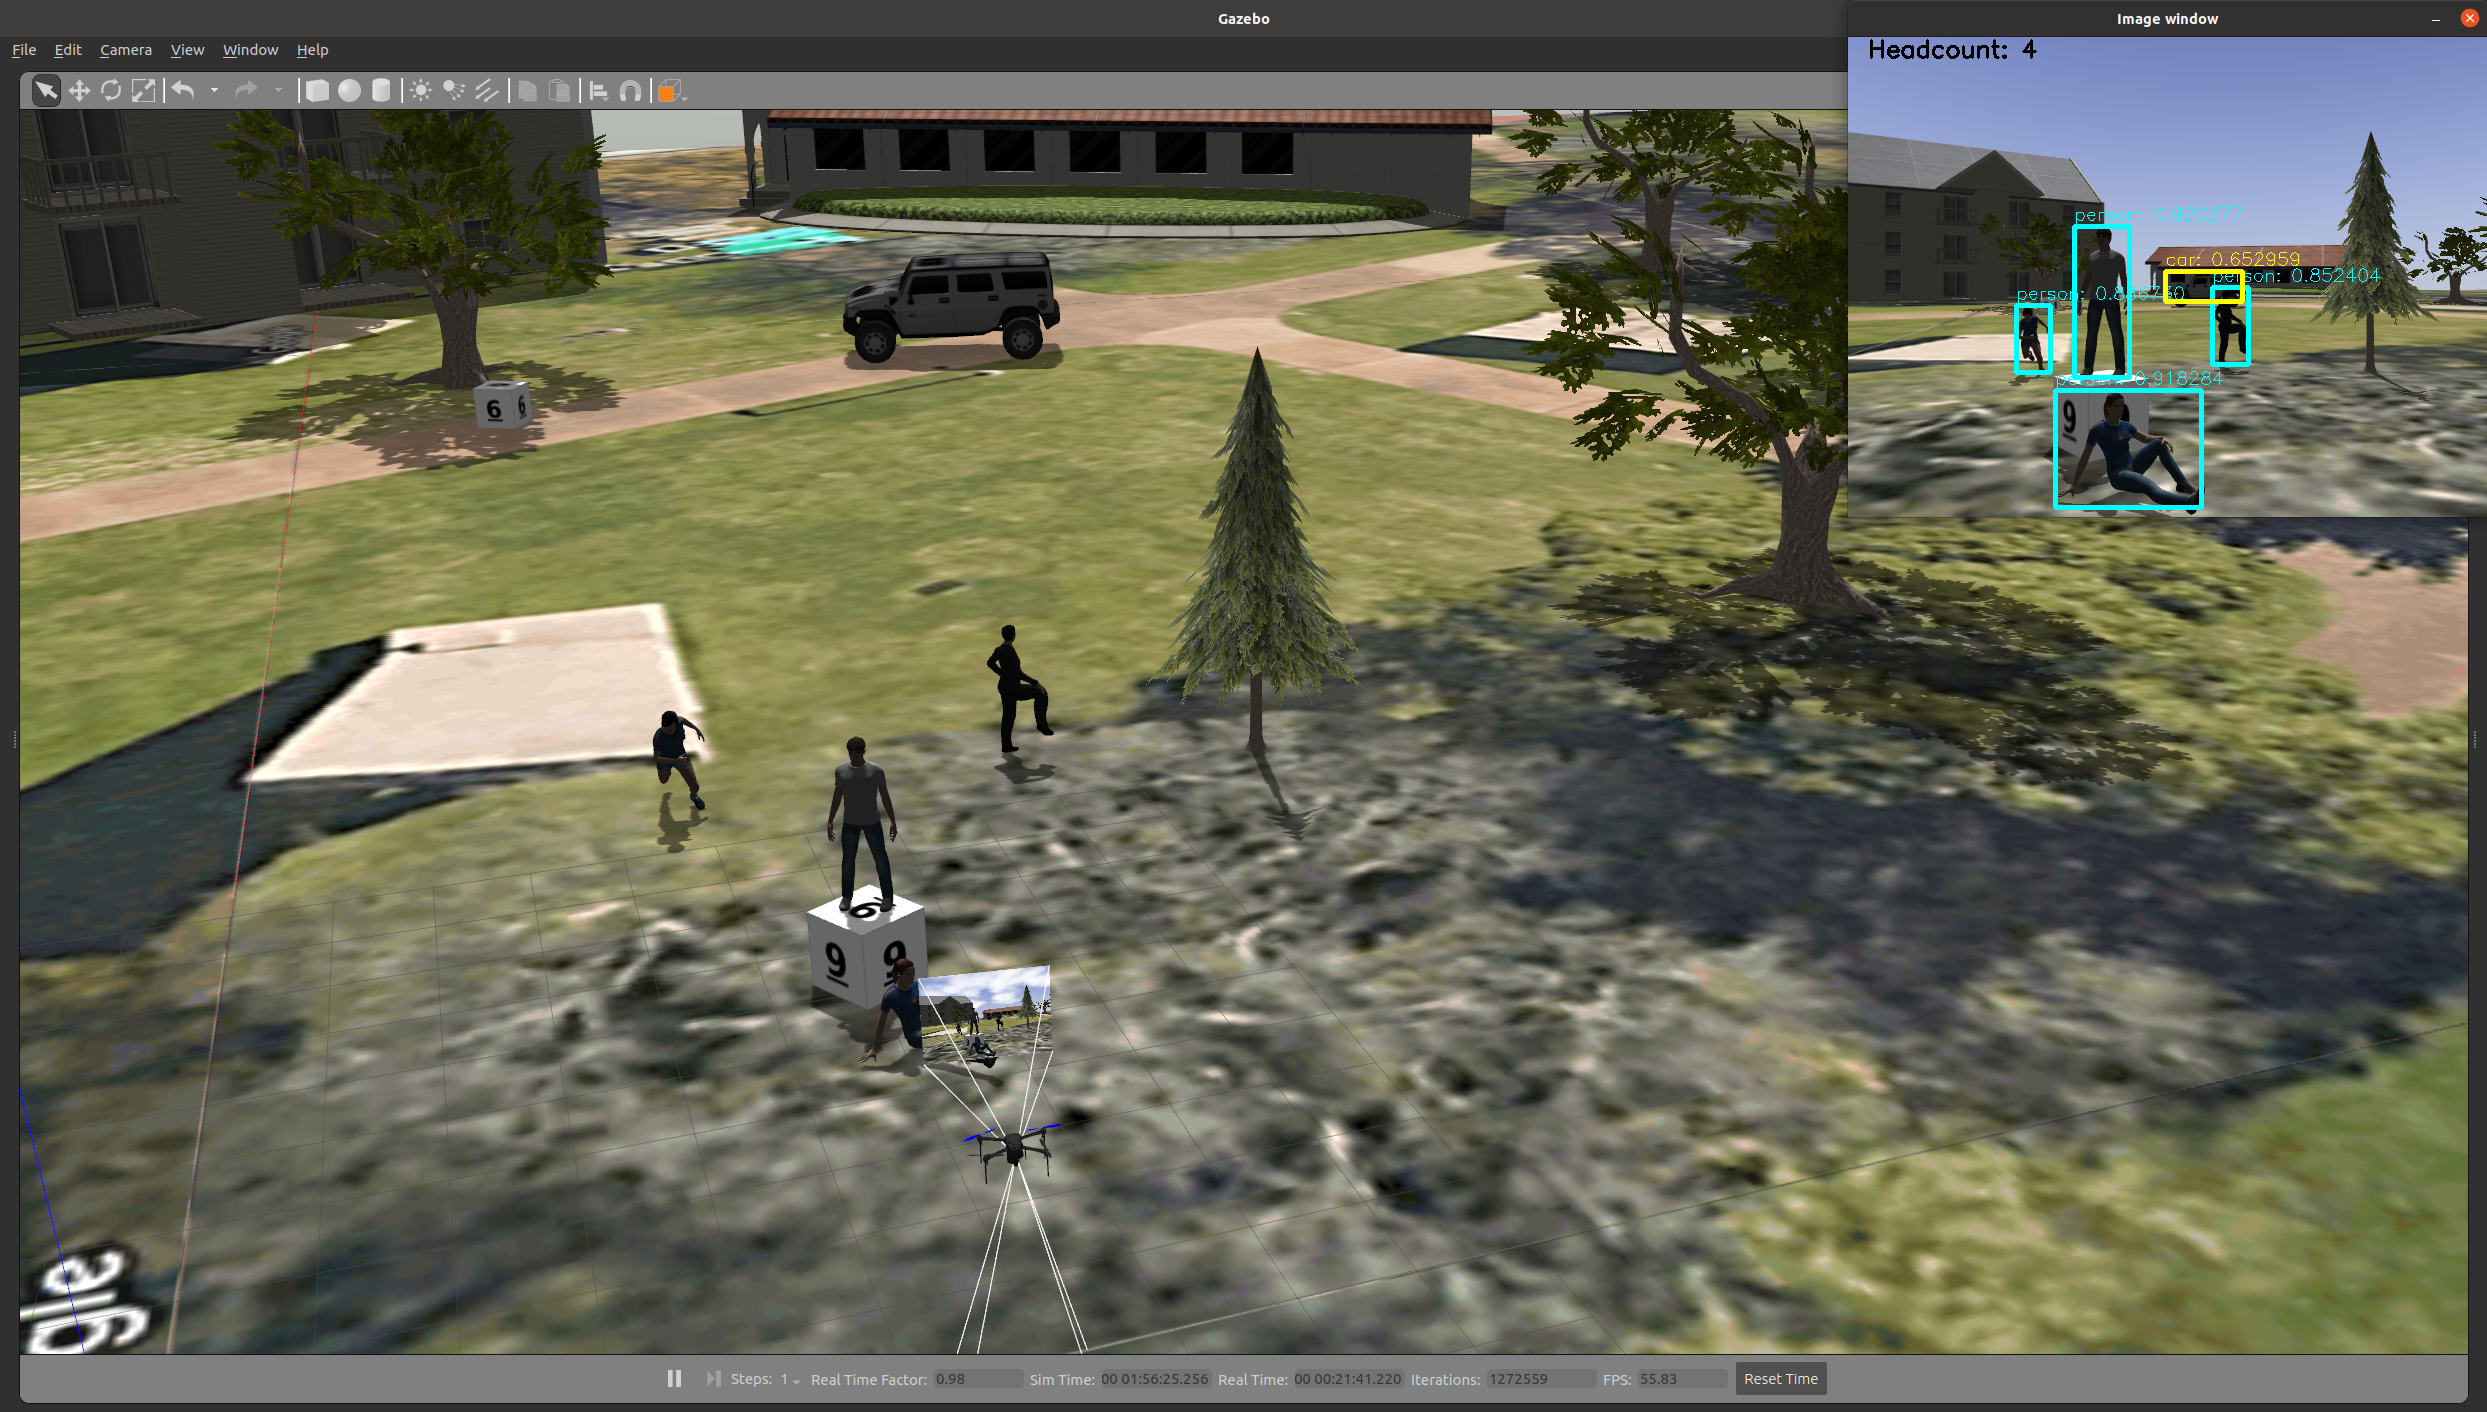
\includegraphics[width=0.5\textwidth]{Figures/Results/headcount.png}}
    \caption{Counting the Number of Humans in the Frame (camera positioned horizontally)}
    \label{fig3d2}
\end{figure}

The final experiment was designed to test the drone's capacity for dynamic human detection within its field of view. In this scenario, the drone was programmed to continuously rotate about its axis until it successfully detected a human model within its camera frame. The drone's software was programmed with algorithms to determine the human's relative position in the frame in real-time and adjust its orientation accordingly. As the drone began rotating, it utilized the integrated camera to scan the environment and processed the data with the YOLO model. The rotation speed was carefully calibrated to ensure sufficient time for image processing and recognition and balance between the agility of response and the accuracy of detection. A demonstration of the successful human tracking task is shown in Fig. \ref{fig3d3}. This result showcases the drone's advanced ability to autonomously identify and focus on human subjects in its environment.

\begin{figure}[H]
    \centerline{\includegraphics[width=0.5\textwidth]{Figures/Results/human_tracking.jpeg}}
    \caption{Human Tracking Task (camera positioned horizontally): Rotate (top left) $\rightarrow$ Rotate (top right) $\rightarrow$ Rotate (bottom left) $\rightarrow$ Stop (bottom right)}
    \label{fig3d3}
\end{figure}